\documentclass[12pt, a4paper, simple]{eskdtext}

\usepackage{config/main.env}
\usepackage{config/report.env}
\usepackage{styles/listing}
\usepackage{styles/lists}
\usepackage{styles/SectionMargins}
\usepackage{styles/table}
\usepackage{styles/TableOfContent}
\usepackage{styles/url}

\begin{document}
  \begin{ESKDtitlePage}
  \ESKDstyle{empty}
  \begin{center}
    \envReportMinistr \\
    \envReportEducation \\
    \envReportUniversity \\
    \envReportCathedra \\
  \end{center}

  \vfill

  \begin{center}
    Тема: <<\envReportTitle>>
  \end{center}

  \vfill

  \begin{center}
    Отчёт лабораторной работы №\envReportLabNumber \\
    по дисциплине \envReportSubject \\
  \end{center}

  \vfill

  \begin{flushright}
    \begin{minipage}[t]{7cm}
      Выполнил: \\
      \envReportStudentInfo \\
      \hspace{0pt} \\
      Проверил: \\
      \envReportTeacherInfo \\
    \end{minipage}
  \end{flushright}

  \vfill

  \begin{center}
    \envReportCity~\ESKDtheYear
  \end{center}
\end{ESKDtitlePage}


  % = = = = = = = = = = = = = = = =
  \ESKDstyle{empty}
  \begin{center}
    \textbf{Отчёт лабораторной работы №\envReportLabNumber}
  \end{center}

  \paragraph{} \textbf{Тема}: <<\envReportTitle>>

  \paragraph{} \textbf{Цель}:
  Разработка приложения, которое станет основой для формирования инфраструктуры из нескольких микросервисов,
  объединенных общей тематикой.
  Знакомство с OpenAPI.

  \paragraph{} \textbf{Что нужно сделать}:

  Написать веб-приложение APP на определенную (согласно варианту задания) тематику.
  Оно должно состоять только из бэкэнда (серверное), предоставлять внешнему миру некоторое API. 

  Хранение данных должно производиться с использованием СУБД MySQL или Postrgres.

  Для непосредственного взаимодействия с вашим приложением разработать описание API в формате OpenAPI,
  и использовать любой, поддерживающий его, клиент, например, Swagger UI.

  Действия приложения логируйте при помощи подходящего для вашего языка/технологии инструмента.

  \paragraph{} \textbf{Ход работы}:

  Swagger UI изображен на рисунках~\ref{fig:swaggerui_1}, \ref{fig:swaggerui_2}, \ref{fig:swaggerui_3}, \ref{fig:swaggerui_4}.

  Примеры параметров, тела запроса и результаты по кодам изображены на рисунках~\ref{fig:more_1},
  \ref{fig:more_2}, \ref{fig:more_3}, \ref{fig:more_4}, \ref{fig:more_5}, \ref{fig:more_6},
  \ref{fig:more_7}, \ref{fig:more_8}, \ref{fig:more_9}, \ref{fig:more_10}, \ref{fig:more_11}.

  \begin{figure}[!h]
    \centering
    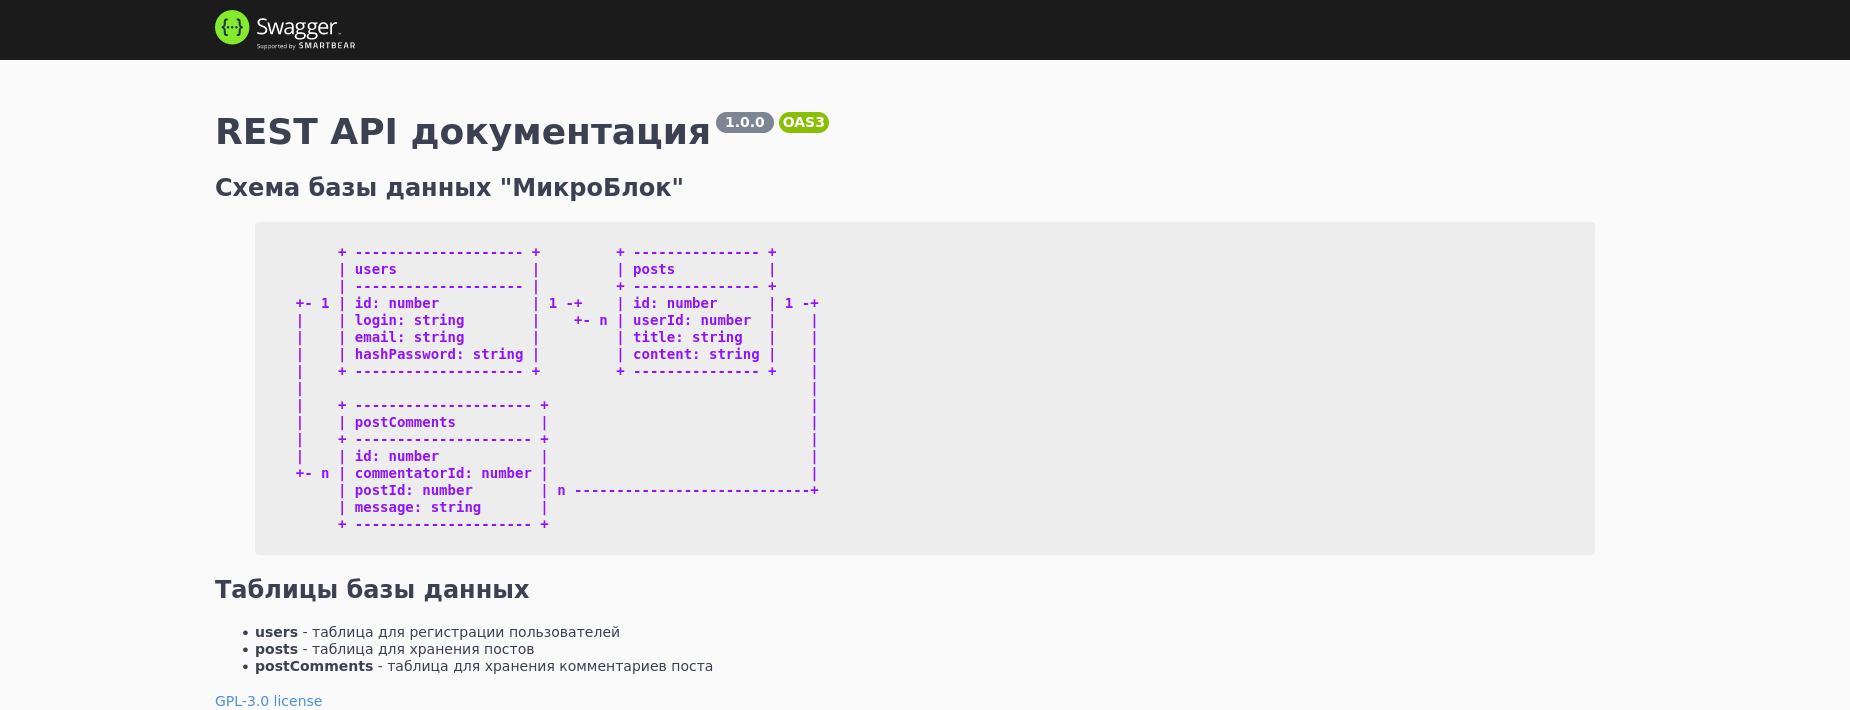
\includegraphics[width=18cm]
    {images/SwaggerUi/2023-02-25_17-57-46.png}
    \caption{Шапка Swagger UI}
    \label{fig:swaggerui_1}
  \end{figure}

  \begin{figure}[!h]
    \centering
    
\includegraphics[width=18cm]
    {images/SwaggerUi/2023-02-25_18-02-00.png}
    \caption{Эндпоинты для работы с пользователями}
    \label{fig:swaggerui_2}
  \end{figure}

  \begin{figure}[!h]
    \centering
    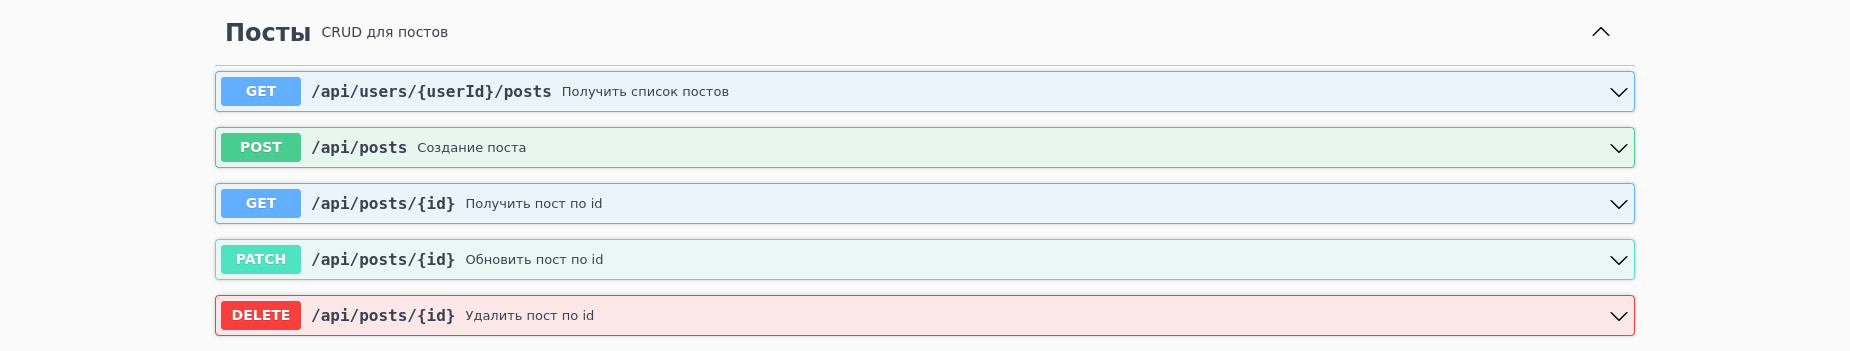
\includegraphics[width=18cm]
    {images/SwaggerUi/2023-02-25_18-03-10.png}
    \caption{Эндпоинты для работы с постами микроблога}
    \label{fig:swaggerui_3}
  \end{figure}

  \begin{figure}[!h]
    \centering
    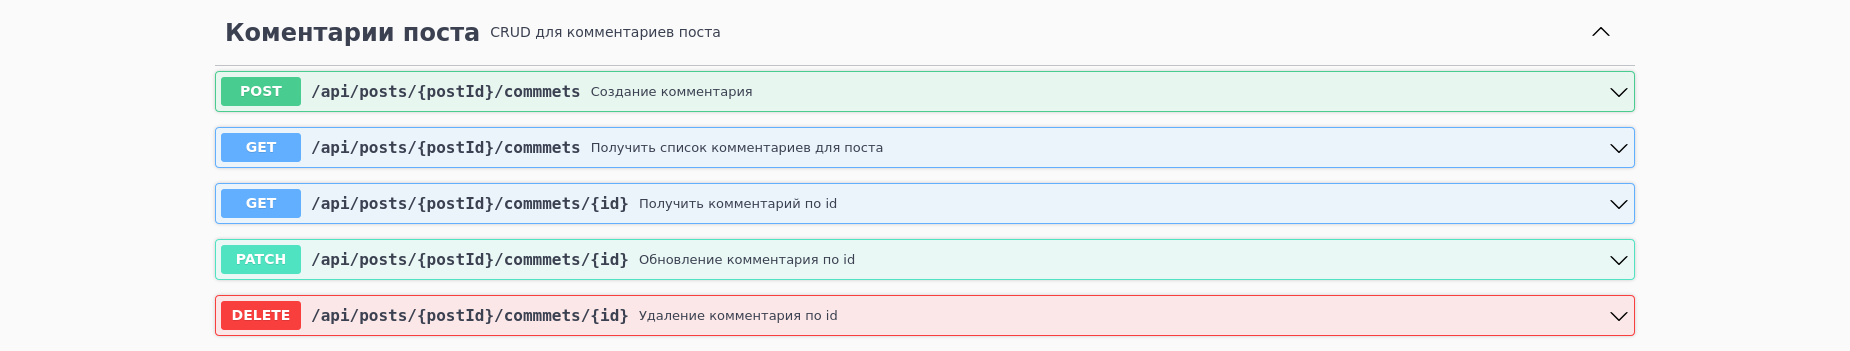
\includegraphics[width=18cm]
    {images/SwaggerUi/2023-02-25_18-04-41.png}
    \caption{Эндпоинты для работы с комментариями постов микроблога}
    \label{fig:swaggerui_4}
  \end{figure}

  \begin{figure}[p!h]
    \centering
    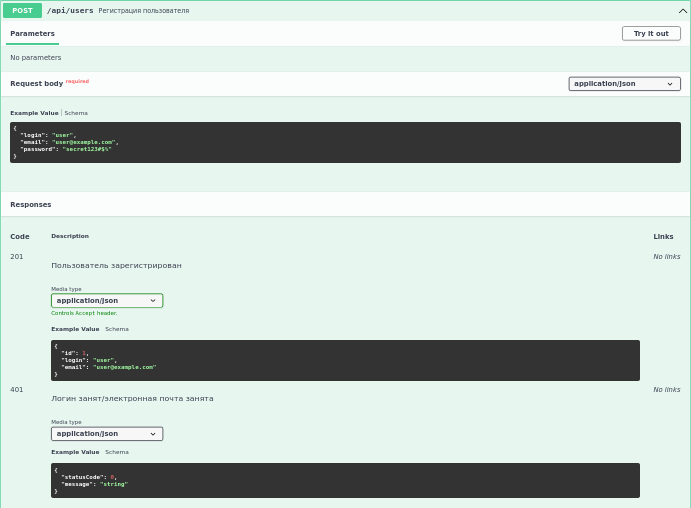
\includegraphics[width=14cm]
    {images/SwaggerUi/2023-02-25_18-06-43.png}
    \caption{Регистрация пользователя}
    \label{fig:more_1}
  \end{figure}

  \begin{figure}[p!h]
    \centering
    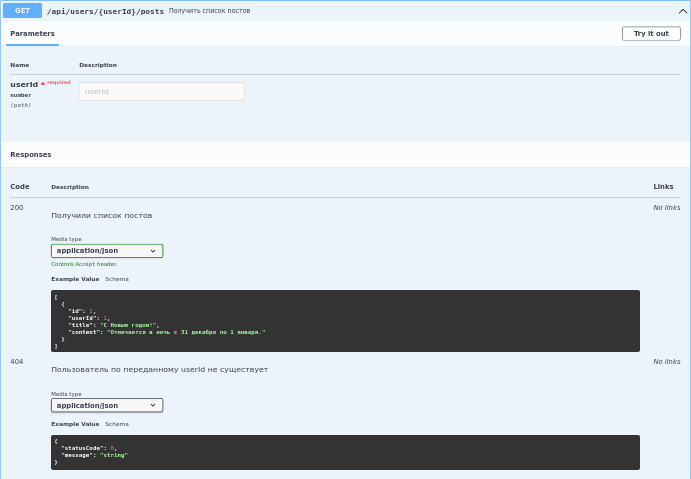
\includegraphics[width=14cm]
    {images/SwaggerUi/2023-02-25_18-07-34.png}
    \caption{Просмотр постов пользователя}
    \label{fig:more_2}
  \end{figure}

  \begin{figure}[p!h]
    \centering
    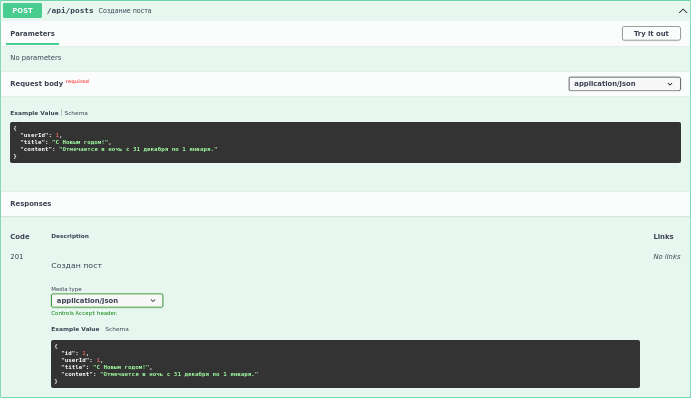
\includegraphics[width=14cm]
    {images/SwaggerUi/2023-02-25_18-08-35.png}
    \caption{Создание поста микроблога}
    \label{fig:more_3}
  \end{figure}

  \begin{figure}[p!h]
    \centering
    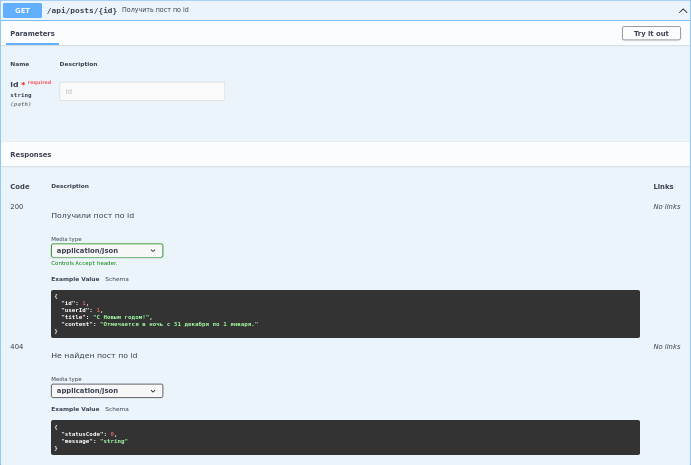
\includegraphics[width=14cm]
    {images/SwaggerUi/2023-02-25_18-09-03.png}
    \caption{Просмотр поста микроблога по ид}
    \label{fig:more_4}
  \end{figure}

  \begin{figure}[p!h]
    \centering
    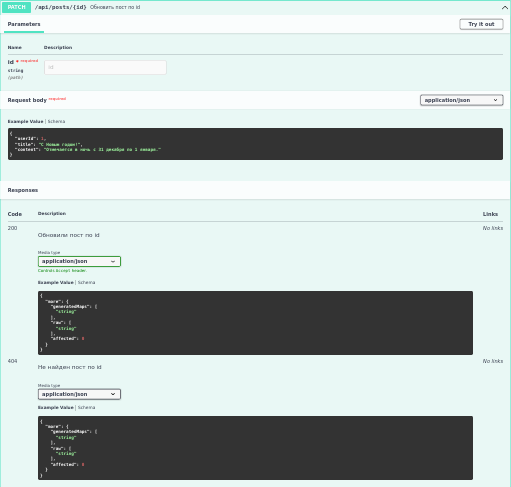
\includegraphics[width=14cm]
    {images/SwaggerUi/2023-02-25_18-10-24.png}
    \caption{Обновление поста микроблога по ид}
    \label{fig:more_5}
  \end{figure}

  \begin{figure}[p!h]
    \centering
    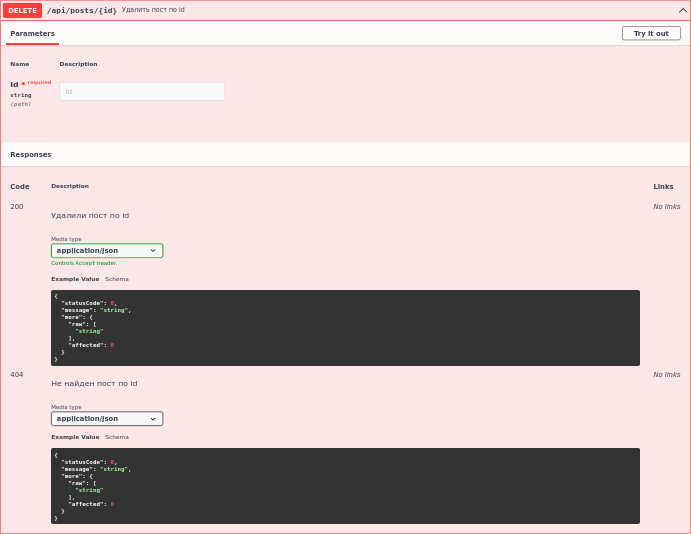
\includegraphics[width=14cm]
    {images/SwaggerUi/2023-02-25_18-10-57.png}
    \caption{Удаление поста микроблога по ид}
    \label{fig:more_6}
  \end{figure}

  \begin{figure}[p!h]
    \centering
    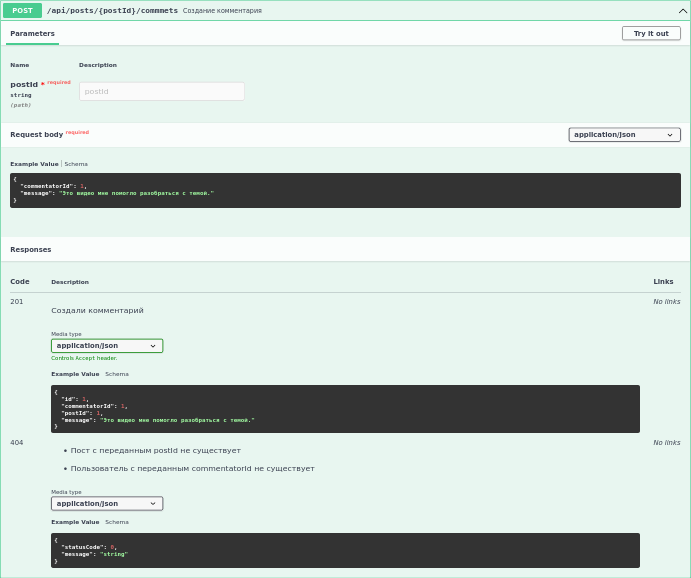
\includegraphics[width=14cm]
    {images/SwaggerUi/2023-02-25_18-13-12.png}
    \caption{Слздание комментария посту микроблога}
    \label{fig:more_7}
  \end{figure}

  \begin{figure}[p!h]
    \centering
    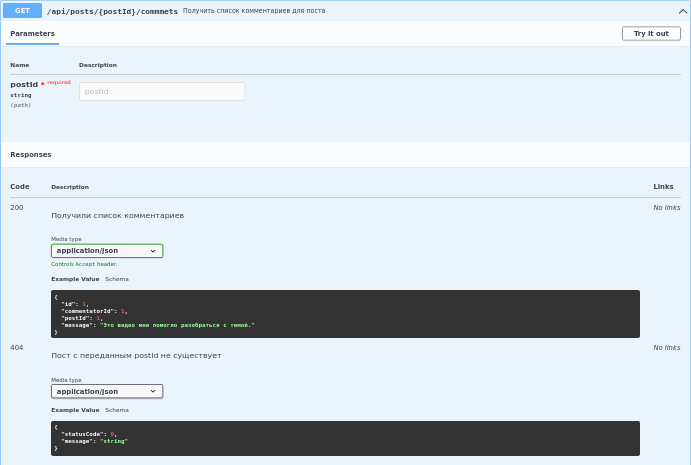
\includegraphics[width=14cm]
    {images/SwaggerUi/2023-02-25_18-14-19.png}
    \caption{Просмотр всех комментарив поста микроблога}
    \label{fig:more_8}
  \end{figure}

  \begin{figure}[p!h]
    \centering
    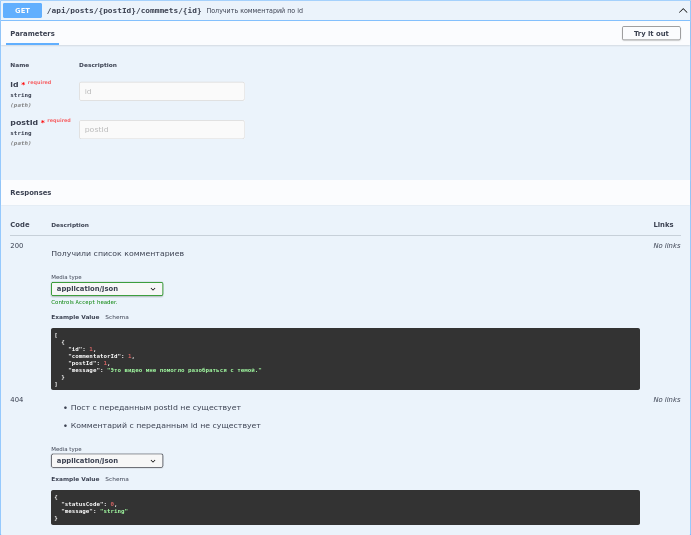
\includegraphics[width=14cm]
    {images/SwaggerUi/2023-02-25_18-14-52.png}
    \caption{Просмотр комментария поста микроблога по ид}
    \label{fig:more_9}
  \end{figure}

  \begin{figure}[p!h]
    \centering
    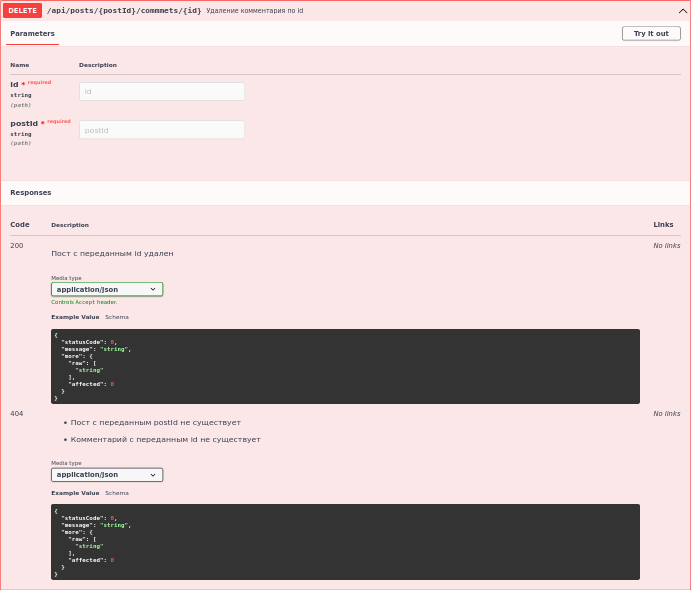
\includegraphics[width=14cm]
    {images/SwaggerUi/2023-02-25_18-15-52.png}
    \caption{Удаление комментария поста микроблога по ид}
    \label{fig:more_10}
  \end{figure}

  \begin{figure}[p!h]
    \centering
    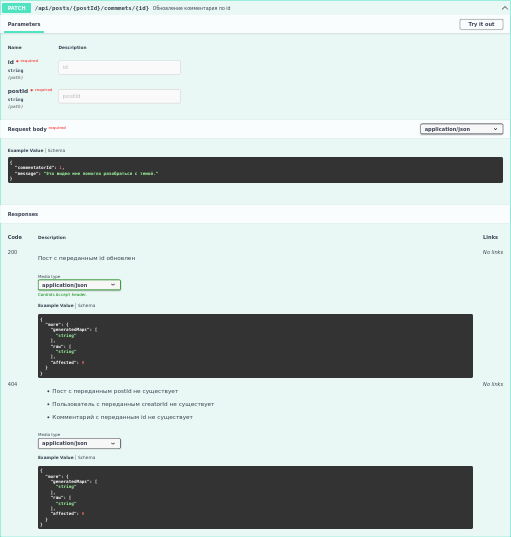
\includegraphics[width=14cm]
    {images/SwaggerUi/2023-02-25_18-15-22.png}
    \caption{Обновление комментария поста микроблога по ид}
    \label{fig:more_11}
  \end{figure}

  \newpage

  \paragraph{} \textbf{Вывод}:
  Написали приложение на NestJS. Записали данные в БД Postgres. Задокументировали API используя SwaggerUI. 

  % = = = = = = = = = = = = = = = =
  \newpage
  \begingroup
    \phantomsection
    \addcontentsline{toc}{section}{СПИСОК ИСПОЛЬЗОВАННЫХ ИСТОЧНИКОВ}
    \section*{Список использованных источников} %\section*{СПИСОК ИСПОЛЬЗОВАННЫХ ИСТОЧНИКОВ}

    \renewcommand{\addcontentsline}[3]{}% Remove functionality of \addcontentsline
    \renewcommand{\section}[2]{}% Remove functionality of \section

    \begin{thebibliography}{}

    \bibitem{typescript_1}
    Урок 1. Установка typescript. Как работает компиляция в ts. Обучение typescript с нуля. - YouTube
    [Электронный ресурс]. -
    Режим доступа:
    \url{https://www.youtube.com/watch?v=TZXDHK0UXZM}.
    Дата доступа: 30.12.2022.

    \bibitem{typescript_2}
    Урок 2. Типы данных typescript: string, number, boolean, undefined, null, any - YouTube
    [Электронный ресурс]. -
    Режим доступа:
    \url{https://www.youtube.com/watch?v=bmalaqfT5xs}.
    Дата доступа: 30.12.2022.

    \bibitem{typescript_3}
    Урок 3. Typescript массивы: Основные методы работы с массивами в Typescript. - YouTube
    [Электронный ресурс]. -
    Режим доступа:
    \url{https://www.youtube.com/watch?v=IBtS6LQgxQE}.
    Дата доступа: 30.12.2022.

    \bibitem{typescript_4}
    Урок 4. Типизация функции typescript, работа с параметрами функции, стрелочные функции - YouTube
    [Электронный ресурс]. -
    Режим доступа:
    \url{https://www.youtube.com/watch?v=yzSX9SNiKEY}.
    Дата доступа: 30.12.2022.

    \bibitem{typescript_5}
    Урок 5. TypeScript object. Типизация объектов в typescript - YouTube
    [Электронный ресурс]. -
    Режим доступа:
    \url{https://www.youtube.com/watch?v=9qaucEQ3XtI}.
    Дата доступа: 30.12.2022.

    \bibitem{typescript_6}
    Урок 6. TypeScript Interface. Как работать с интерфейсами в typescript - YouTube
    [Электронный ресурс]. -
    Режим доступа:
    \url{https://www.youtube.com/watch?v=0DFY_TymPmc}.
    Дата доступа: 30.12.2022.

    \bibitem{typescript_7}
    Урок 7. Как работают литералы в typescript. Literals in typescript - YouTube
    [Электронный ресурс]. -
    Режим доступа:
    \url{https://www.youtube.com/watch?v=2O7Ih4uFb-Y}.
    Дата доступа: 30.12.2022.

    \bibitem{typescript_8}
    Урок 8. Классы в typescript. Модификаторы доступа: public, protected, private, onlyread. Static - YouTube
    [Электронный ресурс]. -
    Режим доступа:
    \url{https://www.youtube.com/watch?v=aKZRBk0u2wE}.
    Дата доступа: 30.12.2022.

    \bibitem{typescript_9}
    Урок 9. Как работать с enum в typescript. Enums typescript - YouTube
    [Электронный ресурс]. -
    Режим доступа:
    \url{https://www.youtube.com/watch?v=xIFVjuAHgFU}.
    Дата доступа: 30.12.2022.

    \bibitem{typescript_10}
    Урок 10. Generics в typescript: function. array, class, interface, type, keyof - YouTube
    [Электронный ресурс]. -
    Режим доступа:
    \url{https://www.youtube.com/watch?v=x5-cYTjX0Po}.
    Дата доступа: 30.12.2022.

    \bibitem{nodejs_nestjs_example}
    Продвинутый BACKEND на Node.js. Nest js ПОЛНЫЙ КУРС \& Docker - YouTube
    [Электронный ресурс]. -
    Режим доступа:
    \url{https://www.youtube.com/watch?v=dDeWWQWMM-Y}.
    Дата доступа: 30.12.2022.

    \bibitem{nestjs_docs}
    Documentation | NestJS - A progressive Node.js framework
    [Electronic resource]. -
    Mode of access:
    \url{https://docs.nestjs.com}.
    Date of access: 12.01.2023.

    \bibitem{docker_without_sudo}
    Как использовать Docker без sudo на Ubuntu
    [Электронный ресурс]. -
    Режим доступа:
    \url{https://itisgood.ru/2020/07/09/docker-compose-dlja-mysql-s-phpmyadmin}.
    Дата доступа: 13.01.2023.

    \bibitem{nestjs_typeorm}
    NestJS TypeORM Repository. Работаем с БД mysql. CRUD операции для REST API - YouTube
    [Electronic resource]. -
    Mode of access:
    \url{https://www.youtube.com/watch?v=BLt9WjWXR3U}.
    Date of access: 14.01.2023.

    \bibitem{nestjs_validation}
    Validation | NestJS — прогрессивный фреймворк Node.js
    [Electronic resource]. -
    Mode of access:
    \url{https://nestjs.ru/techniques/validation}.
    Date of access: 14.01.2023.

    \bibitem{nestjs_validation_annotations}
    typestack/class-validator: Decorator-based property validation for classes.
    [Electronic resource]. -
    Mode of access:
    \url{https://github.com/typestack/class-validator#validation-decorators}.
    Date of access: 14.01.2023.

    \bibitem{nestjs_typeorm_manytomany_1}
    One to Many and Many to One Relations | \#12 | Node Js TypeORM MySql in Hindi - YouTube
    [Electronic resource]. -
    Mode of access:
    \url{https://www.youtube.com/watch?v=capG52wsRfk}.
    Date of access: 15.01.2023.

    \bibitem{nestjs_typeorm_manytomany_2}
    How to create One to Many and Many to Many relationships in TypeORM | by Wilson Matokanovic Junior | Medium
    [Electronic resource]. -
    Mode of access:
    \url{https://medium.com/@wilsonmjuniorx/how-to-create-one-to-many-and-many-to-many-relationships-in-typeorm-473a7d54cb87}.
    Date of access: 20.01.2023.

    \bibitem{nestjs_swagger_apitags}
    How to add description to @ApiTags for swagger in NestJS? - Stack Overflow
    [Electronic resource]. -
    Mode of access:
    \url{https://stackoverflow.com/questions/70709925/how-to-add-description-to-apitags-for-swagger-in-nestjs}.
    Date of access: 20.01.2023.

  \end{thebibliography}
  \endgroup
  % = = = = = = = = = = = = = = = =
\end{document}
